% !TeX program = xelatex

\documentclass[rgb]{article}
\usepackage{themeKonstanz}
\usepackage{pifont,multicol}
%\usepackage{mwe}


\definecolor{titleFrameBlue}{rgb}{0.215, 0.375, 0.5703}
\definecolor{mmcolor}{rgb}{0,0,0}

%%%%%%%%%%%%%%%%%%%%%%%%%% % % %
% Bibliography and references %
%%%%%%%%%%%%%%%%%%%%%%%%%%%%%


\usepackage[backend=biber, style=phys, biblabel=brackets, maxcitenames=2, maxbibnames=2]{biblatex}
\renewbibmacro*{title}{}
\addbibresource{~/library.bib}
\addbibresource{references.bib}
\DeclareSourcemap{\maps[datatype=bibtex,overwrite=true]{\map{
	\step[fieldsource=author,
	match=\regexp{Mattia\s*Mantovani},
	replace=\regexp{\{\\color\{mmcolor\}M.~Mantovani\}}]
}\map{
	\step[fieldsource=journaltitle,
	match=\regexp{Phys.\s*Rev.\s*([A-E,X])},
	replace=PR$1]
	\step[fieldsource=journaltitle,%journaltitle
	match=\regexp{Appl.\s*Phys.\s*Lett.},
	replace=APL]
	\step[fieldsource=journaltitle,%journaltitle
	match=\regexp{Phys.\s*Rev.\s*Lett.},
	replace=PRL]
	\step[fieldsource=journaltitle,%journaltitle
	match=\regexp{Proc.\s*Natl.\s*Acad.\s*Sci.\s*USA},
	replace=PNAS]
	\step[fieldsource=journaltitle,%journaltitle
	match=\regexp{Eur.\s*Phys.\s*J.\s*B},
	replace=EPJB]
	\step[fieldsource=journaltitle,%journaltitle
	match=\regexp{Europhys.\s*Lett.},
	replace=EPL]
	\step[fieldsource=journaltitle,%journaltitle
	match=\regexp{Nature\s*Commun.},
	replace=Nat. Commun.]
	\step[fieldsource=pages,
	match=\regexp{([0-9]*).*},
	replace=$1]
}}}

\DeclareCiteCommand{\litcite}{}{%
\color{discreetBlue}\printnames[author]{author}\addcomma\addthinspace{}%
\printfield{journaltitle}\addthinspace{}\printfield{volume}\addcomma\addthinspace{}\printfield{pages}\addthinspace{}\printfield{year}\addperiod}{; }{}


\newcommand{\printshortdate}{\printfield{year}}
\DeclareCiteCommand{\litciteshort}{}{%
\color{discreetBlue}\printnames[author]{author}\addcomma\addthinspace{}%
\printfield{journaltitle}\addthinspace{}\printfield{volume}\addthinspace{}\printshortdate\addperiod}{; }{}

\DefineBibliographyStrings{english}{%
    andothers = {\em et\addabbrvspace al\adddot}
}

\renewcommand*{\bibfont}{\fontsize{24}{28.8}}


%%%%%%%%%%%%%%%%%%%%%%%%%%
% Commands and variables %
%%%%%%%%%%%%%%%%%%%%%%%%%%

\renewcommand{\unilogo}[1][UniKonstanz_Logo.pdf]{%
	\begin{textblock*}{\paperwidth}(0cm, 2cm)%
		\rightskip 2cm
		\hfill\includegraphics[scale=1.5]{#1}
	\end{textblock*}%
}%

\newcommand{\bluebf}[1]{\textcolor{seeblau100}{\textbf{#1}}}
\newcommand{\orangebf}[1]{\textcolor{amber}{\textbf{#1}}}
\newcommand{\pinkbf}[1]{\textcolor{pink}{\textbf{#1}}}
\newcommand{\greybf}[1]{\textcolor{schwarz60}{\textbf{#1}}}
\newcommand{\redbf}[1]{\textcolor{alizarin}{\textbf{#1}}}
\newcommand{\magentabf}[1]{\textcolor{magenta}{\textbf{#1}}}
\newcommand{\greenbf}[1]{\textcolor{green!30!black!90}{\textbf{#1}}}

\renewcommand{\Rightarrow}{\text{\color{seeblau100}\ding{220}}}
\newcommand{\bitem}{\item[\color{seeblau100}$\scriptstyle\blacksquare\;$]}



 
%%%%%%%%%
% Paths %
%%%%%%%%%
\makeatletter
\def\input@path{{./blocks/}}
\makeatother
\graphicspath{{./graphics/}}


\format{a0}

\setmainfont{Arial}
\setsansfont{Arial}
\setmathsfont(Digits,Latin,Special){Arial}


%====================================
% Define Frames
%====================================
\newcounter{frameidcounter}
\newcommand*\showframeid{
\begin{tikzpicture}[remember picture,overlay]
	\foreach \x in {1,...,\arabic{frameidcounter}}
	\node[anchor=north west,fill=red,text=white,draw,minimum size=2em] at (frameid \x.north west) {\Large \x};
\end{tikzpicture}
}
\newenvironment{pframe}[1][0.30]{
	\begin{tikzpicture}[remember picture]
	\refstepcounter{frameidcounter} 
 	\node[draw=titleFrameBlue,rounded corners=0em, line width=2pt,fill=white, inner sep=1em,fill opacity=0.9](frameid \arabic{frameidcounter})\bgroup%
	\begin{minipage}[t]{#1\textwidth}
}{
	\end{minipage}\egroup;
	\end{tikzpicture}
}


%%%%%%%%%%%%%%%%%%%%%%%%%%%%%%%%
% Beginning of poster          %
%%%%%%%%%%%%%%%%%%%%%%%%%%%%%%%%

\begin{document}






\newlength{\titleheight}
\newlength{\headerheight}
\newlength{\introheight}
\newlength{\modelheight}
\newlength{\coolingheight}
\newlength{\transferheight}
\newlength{\blockxsep}
\newlength{\blockysep}
\newlength{\margin}

\setlength{\blockxsep}{1cm}
\setlength{\blockysep}{1cm}
\setlength{\margin}{2cm}


\newcommand{\titleblock}{
	\selectfontsize{82pt}
	\markieren{\textbf{Single-atom laser and single-photon pump}}{\textbf{in quantum-dot-based hybrid nanodevices}}{}{}
}


\newcommand{\header}{
\unilogo
% ==== TITLE ==== %
\begin{textfeld}{\margin}{\margin}%
	\titleblock
\end{textfeld}%
\settoheight{\titleheight}{\vbox{\titleblock}}


%% ==== ZUKO LOGO ==== %
%\begin{textfeld}{0cm}{\margin}%
%	\rightskip 25cm
%	\hfill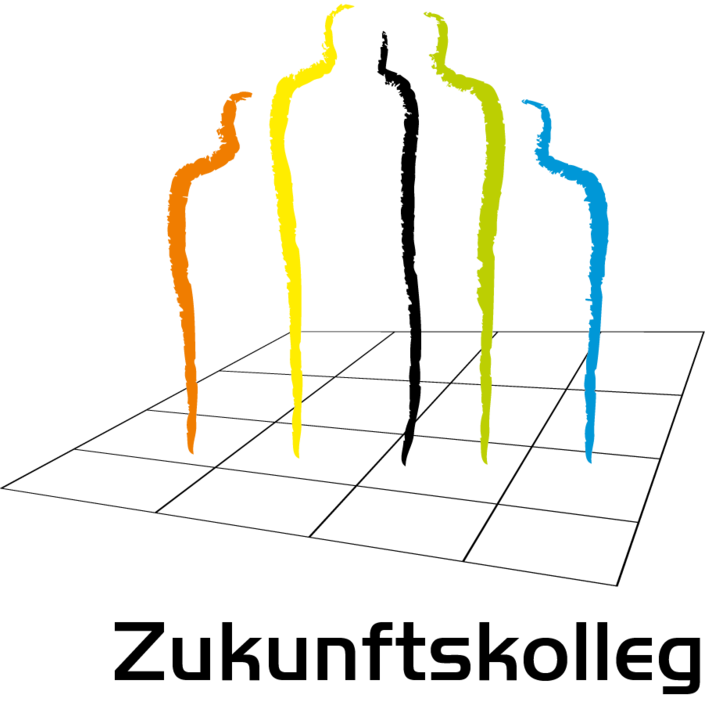
\includegraphics[scale=1.5]{graphics/Zukunftskolleg_Logo.png}
%\end{textfeld}%

% ==== SFB LOGO ==== %
\begin{textfeld}{0cm}{12.5cm}%
	\rightskip \margin
	\hfill
\includegraphics[scale=0.8]{graphics/sfb767_Logo.png}
\end{textfeld}%
\selectfontsize{50pt}
\begin{textfeld}{\margin}{\titleheight+3.5cm}
\underline{\textbf{M. Mantovani}}\rlap{,}\textsuperscript{1} 
A. Armour\rlap{,}\textsuperscript{2}
R. Hussein\rlap{,}\textsuperscript{1}
W. Belzig\rlap{,}\textsuperscript{1} and
G. Rastelli\textsuperscript{1,3}
\quad\quad\quad 
\selectfontsize{64pt}
\underline{\textbf{Project C03}}\\[1.5cm]
\selectfontsize{40pt}
\textsuperscript{1}Fachbereich Physik and \textsuperscript{3}Zukunftskolleg, 
Universität Konstanz, D-78457 Konstanz, Germany\\
\textsuperscript{2}School
of Physics and Astronomy, University of Nottingham, Nottingham NG7 2RD, United Kingdom
\\[1.3cm]
\selectfontsize{30pt}
\cdline[thick=12pt]{\paperwidth-20cm}
\end{textfeld}
}
\selectfontsize{24pt}%


\newcommand{\introduction}{ %
	\cdblock[width=\paperwidth-2\margin, columnnum=2, columnspace=0pt, inner=long, 
	block=true]{\selectfontsize{30pt}\underline{\textbf{Introduction}}}{
	\raggedright
	\textbf{Motivation:}\\[1ex]
	\begin{itemize}
	\item \bluebf{Hybrid devices} (quantum dots + harmonic cavities) offer a 
	playground
	to engineer coherent interactions at the nanoscale~\cite{Viennot2014,Stockklauser2017}\\[0.5ex]
	%
	\item \bluebf{Cooper-pair splitters} (CPSs) are a natural source of 
	entangled 
	electrons, which can be used to induce \bluebf{nonlocal 
	correlations}~\cite{Schindele2012}\\[0.5ex]
	%
	\item Combining these elements can lead to new mechanisms of \bluebf{heat 
	exchange} in 
	nanodevices~[4]\\[1ex]
	\end{itemize}
	%
	\begin{center}
		\begin{multicols}{2}
	%	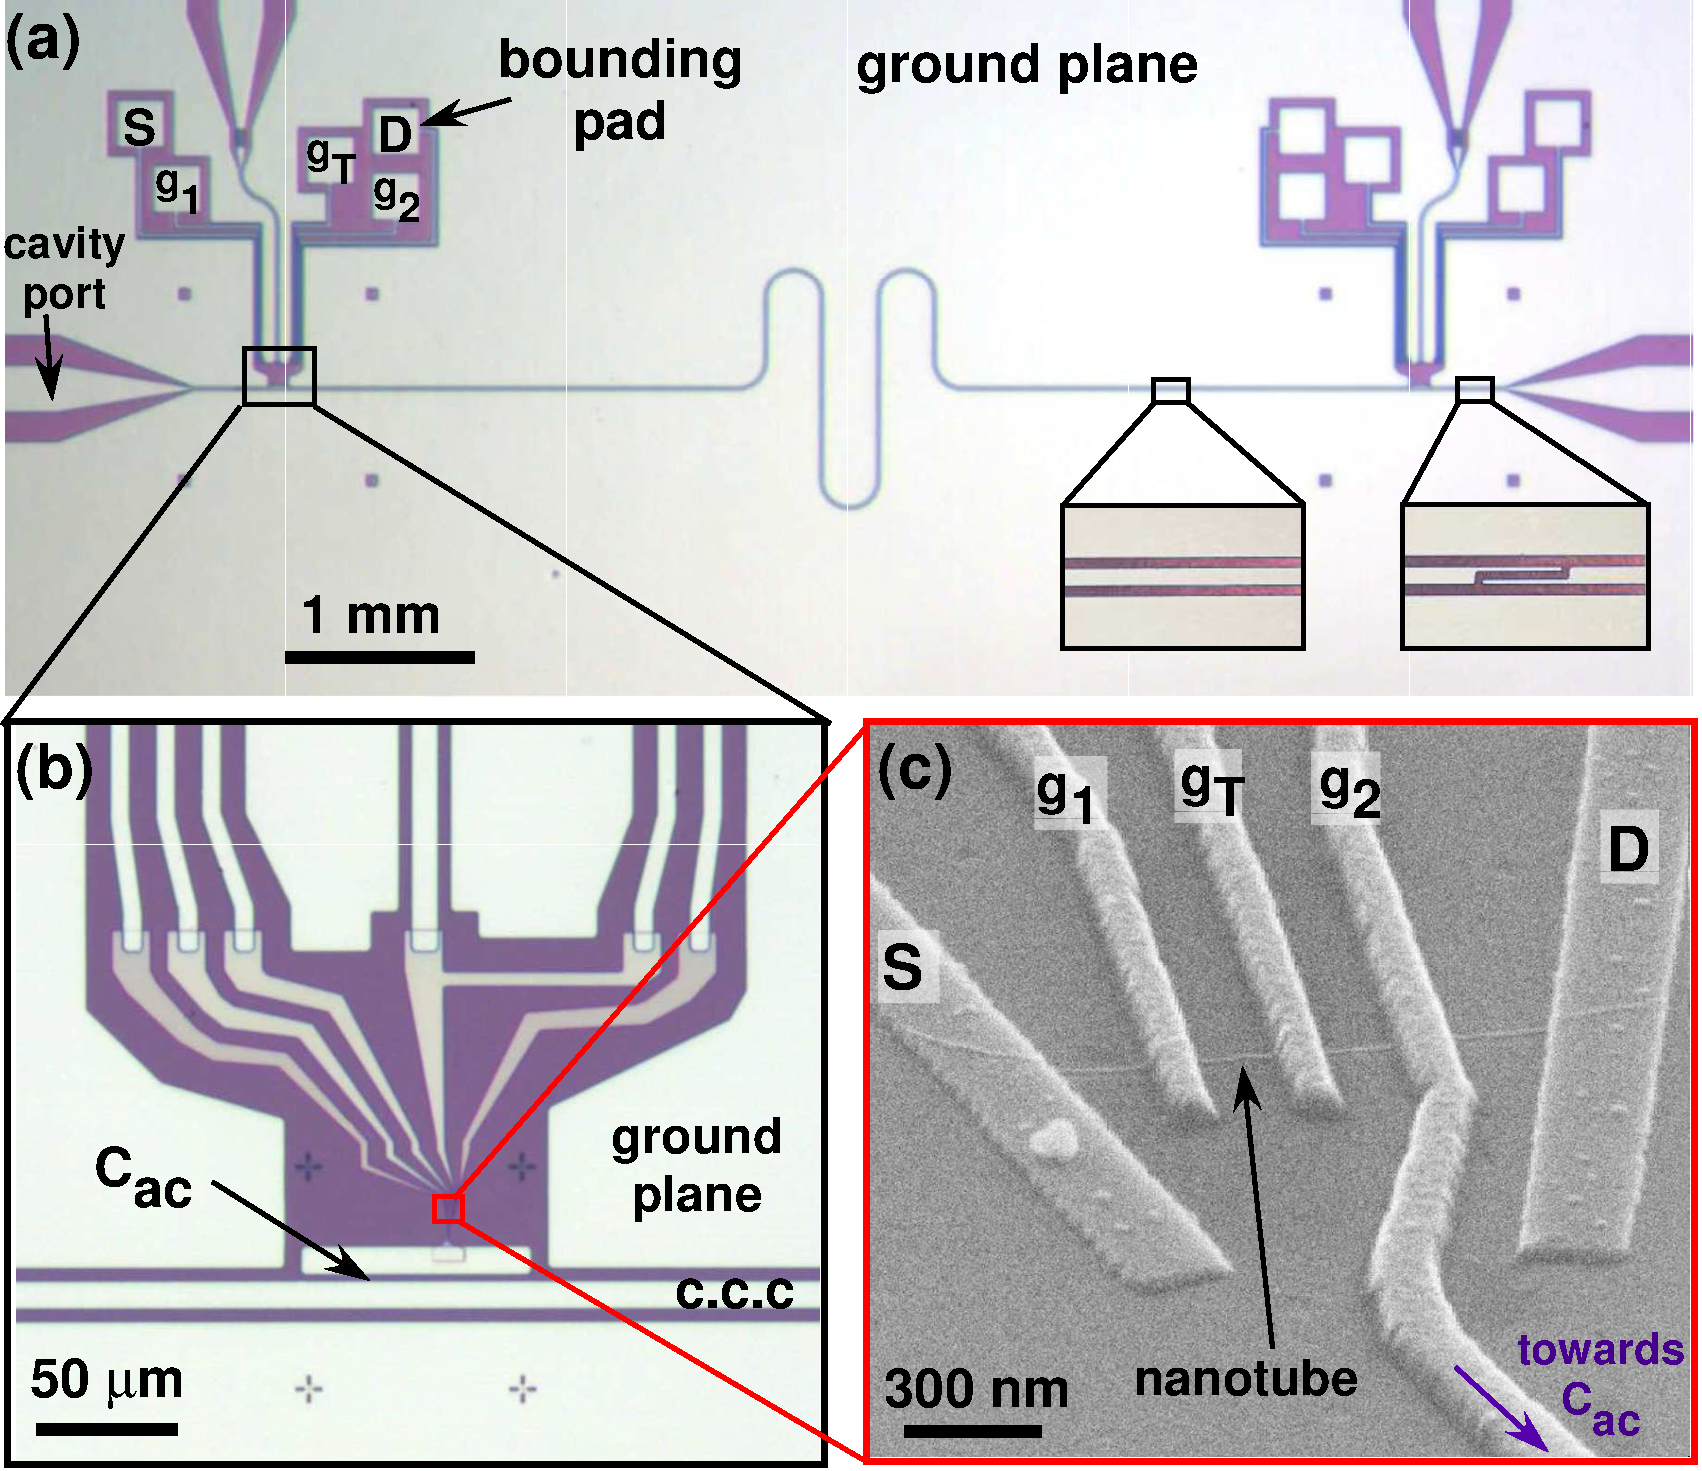
\includegraphics[height=0.3\textwidth]{Cottet2017.pdf}
	%	\newpage %
	%	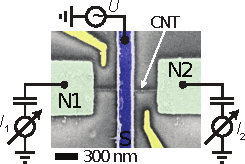
\includegraphics[height=0.3\textwidth]{SchindelePRL2012aFig1b.pdf}
		\end{multicols}
	\end{center}
	%
	\begin{center}
		\begin{multicols}{2}
		Viennot et al., PRB '14
		\newpage
		Schindele et al., PRL '12
		\end{multicols}
	\end{center}
	\vspace{1em}
	\textbf{Here:} CPS with two quantum dots (QDs) and local coupling to two 
	harmonic oscillators (microwave cavities or nanomechanical 
	resonators)~[5]\\[2.8ex]
	
	%
	\underline{\textbf{Main results:}}\\[2.8ex]
	%
	\begin{itemize}
		\item \bluebf{Simultaneous ground-state cooling} of both 
		cavities\\[1ex]
		\item \bluebf{Nonlocal energy transfer} between the two 
		resonators\\[3ex]
	\end{itemize}
	%
	
	
	}{}{}{}{}{}{}{}
}



\newcommand{\model}{ %
	\cdblock[width=\paperwidth-2\margin-\blockxsep-29cm,columnnum=2, 
	columnspace=1cm, inner=long,
	block=true]{\selectfontsize{30pt}\underline{\textbf{Quantum-dot-based 
	Cooper-pair splitter with coupling to resonators}}}
	{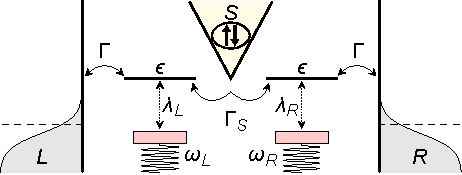
\includegraphics[width=\blockcolumnwidth-0.5cm]{schematics/schematics.pdf}\\[1cm]
	\textbf{System:}
	
	\begin{itemize}
		\item central \orangebf{superconductor} proximizing two QDs: Cooper-pair splitting and recombination with amplitude $\Gamma_S$
		\item QDs tunnel-coupled to negatively biased \greybf{normal leads} 
		\mbox{($L$ and 
		$R$)}
		\item Each QD is capacitively coupled to a \pinkbf{local resonator} 
		(e.g.: microwave cavity or mechanical resonator)\\[2ex]
	\end{itemize}
	%
   \begin{center}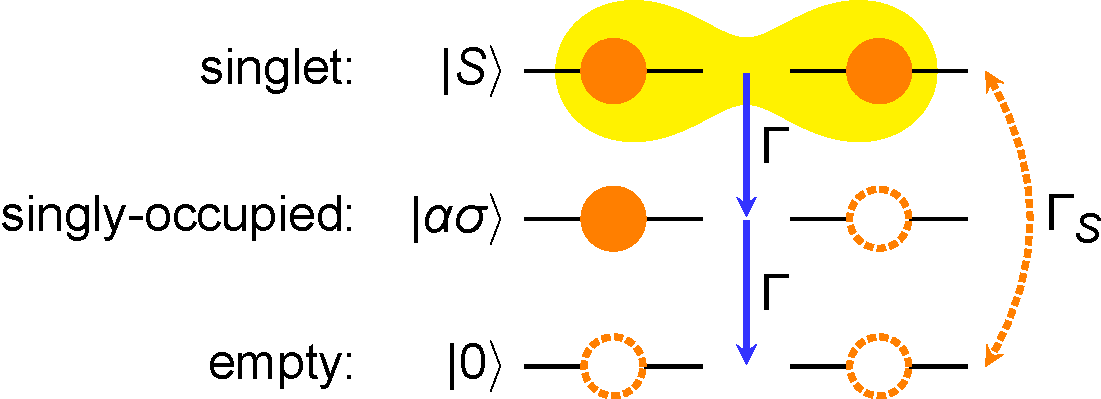
\includegraphics[]{andreev/andreev.pdf}\\[1ex]
   Coherent coupling between $|0\rangle$ and $|S\rangle$:\\ 
   $\Rightarrow$ \orangebf{Andreev bound states}: $|\pm \rangle$
   \end{center}
	}
	{\textbf{Regime:}
	\begin{itemize}
		\item large superconducting gap: $\Delta \rightarrow \infty$
		\item large intradot Coulomb repulsion: $U \rightarrow \infty$
		\item \bluebf{large bias limit}: $k_B T, \epsilon, \Gamma_S \ll e V \ll U, 
		\Delta$ 
    \cdbracket[mode=bottom, 
	arrowleft=false]{\blockcolumnwidth-3cm}{0.2cm}\\[0cm]
	\hskip 0.5\blockcolumnwidth
	\cdline[mode=vertical,arrowright=true]{1cm}\\[0cm]
	\begin{center}\bluebf{cross-Andreev reflection}
	dominates:\\ Cooper pairs 
	are split into 
	separate QDs and tunnel into the leads\\[1cm]
	\end{center}
	\item Single-electron tunneling regime (tunneling rate $\Gamma$) 
    \item Resonators with large quality factors\\[3ex]
	\end{itemize}
	
	\textbf{Effective Hamiltonian} ($\alpha=L,R$, spin index 
	$\sigma=\uparrow,\downarrow$)~[4,6]:
	\begin{equation}
	\begin{split}
		H = &\sum_{\alpha\sigma} \epsilon N_{\alpha\sigma} - 
		\frac{\Gamma_S}{2}(d^\dagger_{R\uparrow} d^\dagger_{L\downarrow} - 
		d^\dagger_{R\downarrow} d^\dagger_{L\uparrow} + \mathrm{H.c.}) + \\
		&\sum_\alpha \omega_\alpha b_\alpha^\dagger b_\alpha + 
		\sum_{\alpha\sigma} \lambda_\alpha(b_\alpha + b_\alpha^\dagger) 
		N_{\alpha\sigma}\nonumber
	\end{split}
	\end{equation}
	\\[2ex]
	%
	\textbf{Methods:}
		\begin{itemize}
			\bitem transition rates $w_{j\leftarrow i}$ between system eigenstates calculated by Fermi Golden Rule
			\bitem Master equation for eigenstate populations~[7,8]: 
			$\dot{P_i} = \sum_j (w_{i\leftarrow j} P_j - w_{j\leftarrow i} 
			P_i)$
			\bitem \bluebf{Numerical solution} for steady populations $\Rightarrow$ average electron currents $I_\alpha$, cavity populations $\bar{n}_\alpha$, and photon energy currents $\dot{E}_\alpha$
		\end{itemize} 
	}
	{}
	{}
	{}
	{}
	{}
	{}
}
%
%
%
%
\newcommand{\cooling}{ %
	\cdblock[width=\paperwidth-2\margin,columnnum=3, 
	columnspace=1cm, 
	block=true,inner=long]{\selectfontsize{30pt}\underline{\textbf{Simultaneous cooling 
	of resonator modes}}}
	{
	%
	Energy splitting of Andreev states: $\delta = \sqrt{\smash[b]{4\epsilon^2 
	+ 2 
	\Gamma_S^2}}$\\[2ex]
	$|\epsilon| \gtrsim \Gamma_S$ $\Rightarrow$ weak charge 
	hybridization\\[2ex]
	\begin{itemize}
		\item $\epsilon > 0$ $\Rightarrow$ $|+\rangle \approx |S\rangle, 
		|-\rangle \approx |0\rangle$
		\item $\epsilon < 0$ $\Rightarrow$ $|+\rangle \approx |0\rangle, 
		|-\rangle \approx |S\rangle$\\[2ex]
	\end{itemize}

	For $\color{blue}{\epsilon > 0}$:\\[2ex]
	\begin{center}
		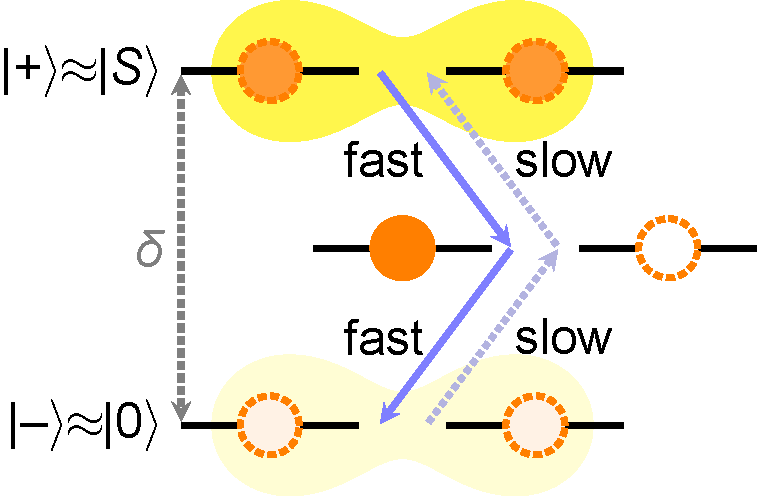
\includegraphics[]{asymm/asymm.pdf}\\[2ex]
	\end{center}
	%
	$\Rightarrow$ weak hybridization yields strong \bluebf{asymmetry} in the 
	transition rates\\
	$\Rightarrow$ the effective interaction with the resonators 
	\bluebf{couples the 
	Andreev states} and leads to interesting effects on the cavities 	
	}
	{
		\begin{itemize}
			\item \underline{\textbf{Case:}} equal frequencies of the modes 
			$(\omega_L = \omega_R)$\\[2ex]
		\end{itemize}
	\textbf{Effective interaction close to $\delta = 
	\omega_\alpha$}:\\[0.5ex]
	\begin{equation}
		H_\mathrm{loc} = \sum_{\alpha} 
		{\color{pink}{\frac{\lambda_\alpha\Gamma_S}{\sqrt{2} 
		\delta}}} (b_\alpha |+\rangle \langle- | + b_\alpha^\dagger |-\rangle 
		\langle + |)\nonumber
	\end{equation}\\[2ex]
	\textbf{Energy diagram:}\\[2ex]
	\begin{center}
				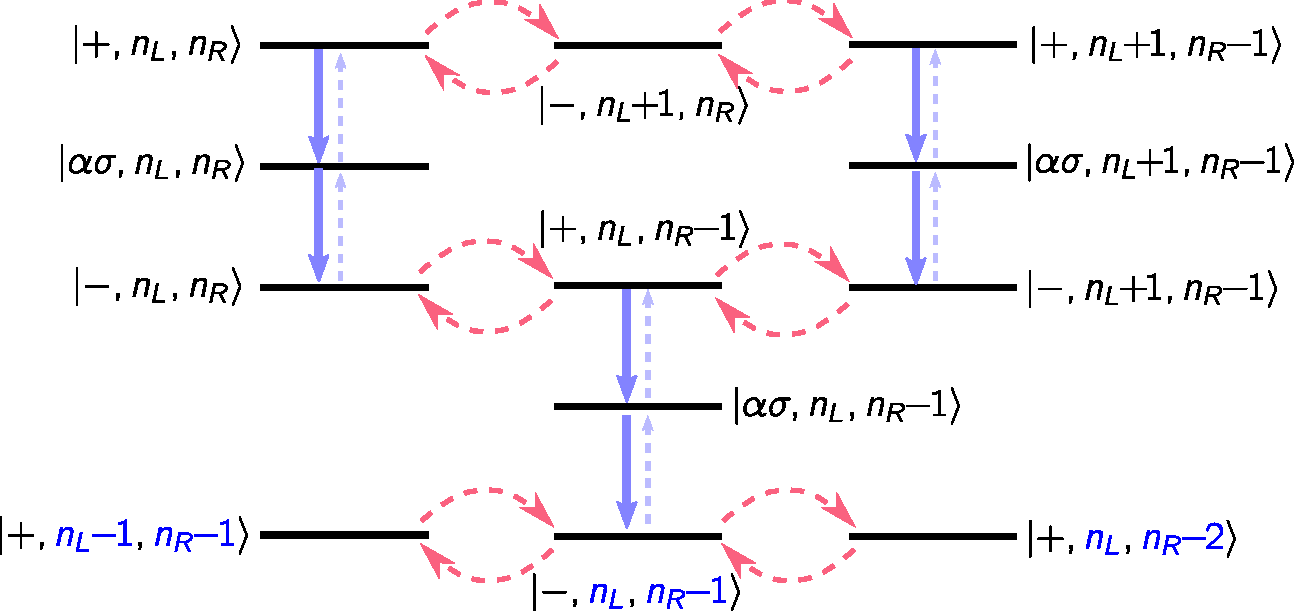
\includegraphics[]{cooling/drawing.pdf}\\[3ex]
	\end{center}
	\begin{itemize}
		\item \pinkbf{Coherent interaction} + 
		\textbf{\textcolor{blue}{electron tunneling}}\\
		$\Rightarrow$ \bluebf{absorption} of one photon per cycle from 
		each cavity
	\end{itemize}
		
	}
	{
	\textbf{Electron current and photon occupation:}\\[2ex]
	\begin{center}
		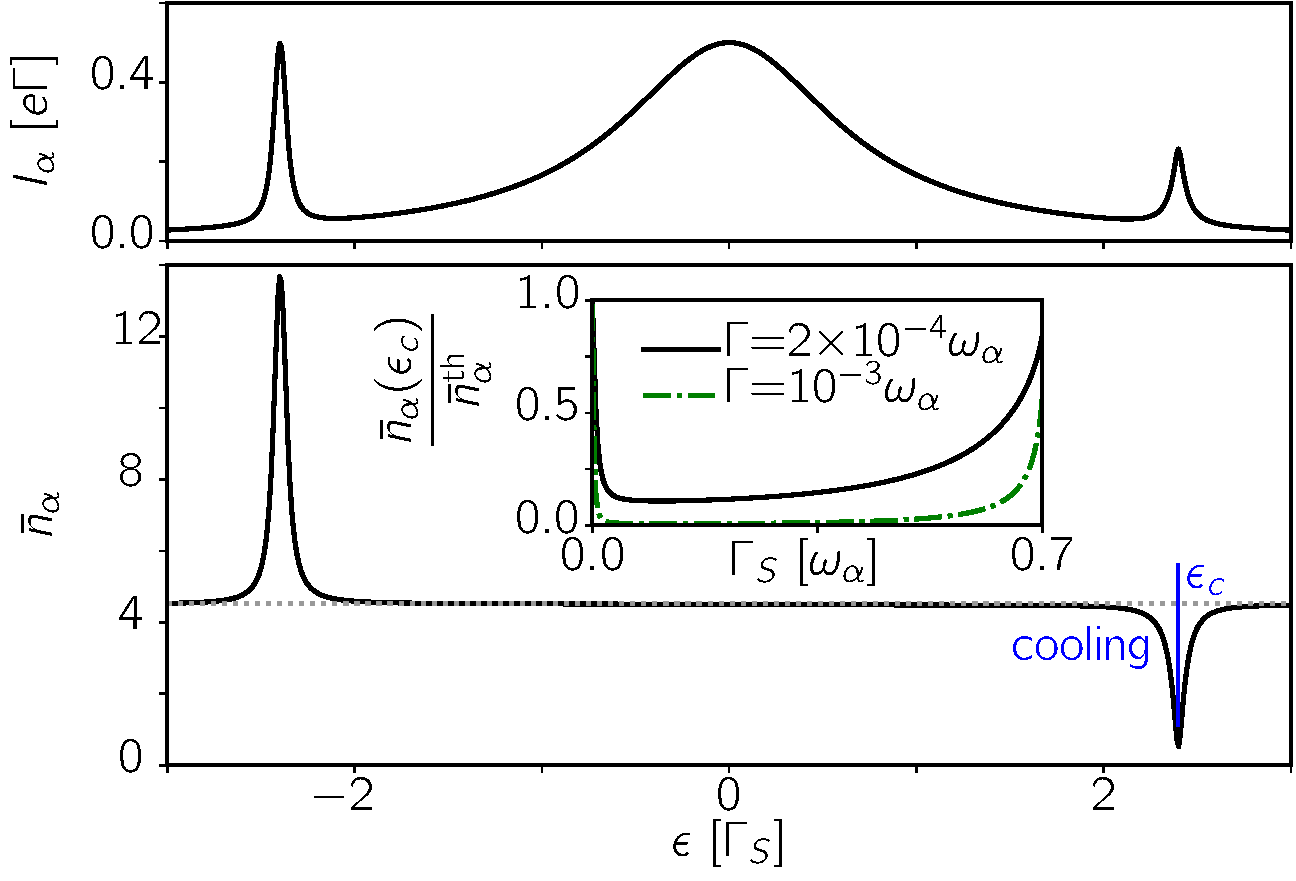
\includegraphics[width=22cm,height=15cm]{Fig2/Fig2.pdf}\\[3ex]
	\end{center}
	\begin{itemize}
	\bitem \textbf{Inelastic peaks} in the electronic current:\\ photon 
	emission or absorption
	\bitem \bluebf{cooling} resonance: $\epsilon_c \approx \frac{1}{2}\sqrt{\smash[b]{\omega_\alpha^2 - 2 \Gamma_S^2}}$
	\bitem \redbf{heating} at $\epsilon = -\epsilon_c$
	\bitem \bluebf{ground-state cooling} is achievable for small values of $\Gamma_S$
	\end{itemize}

	}
	{}
	{}
	{}
	{}
	{}
}

\newcommand{\transfer}{ %
	\cdblock[width=\paperwidth-2\margin,columnnum=3, 
	columnspace=1cm, 
	block=true,inner=long]{\selectfontsize{30pt}\underline{\textbf{Nonlocal photon and 
	heat transfer}}}
	{\begin{itemize}
			\item \underline{\textbf{Case:}} different frequencies of the modes $(\omega_L > \omega_R)$\\[3ex]
		\end{itemize}
\textbf{Operating resonance:} $\delta \approx \omega_L - \omega_R$\\[1ex]
\textbf{Effective Hamiltonian:}
\begin{equation}
	H_\mathrm{NL} = {\color{green!30!black!90}{\lambda_\mathrm{NL}}} 
	(b_L^\dagger b_R |-\rangle \langle+ | + b_L b_R^\dagger |+\rangle \langle- 
	|),\qquad\qquad 
	{\color{green!30!black!90}{\lambda_\mathrm{NL}\approx \frac{\Gamma_S 
	\epsilon}{\delta} 
	\frac{\lambda_L 
	\lambda_R}{\omega_L \omega_R}}}\nonumber
\end{equation}\\[2ex]
\begin{center}
	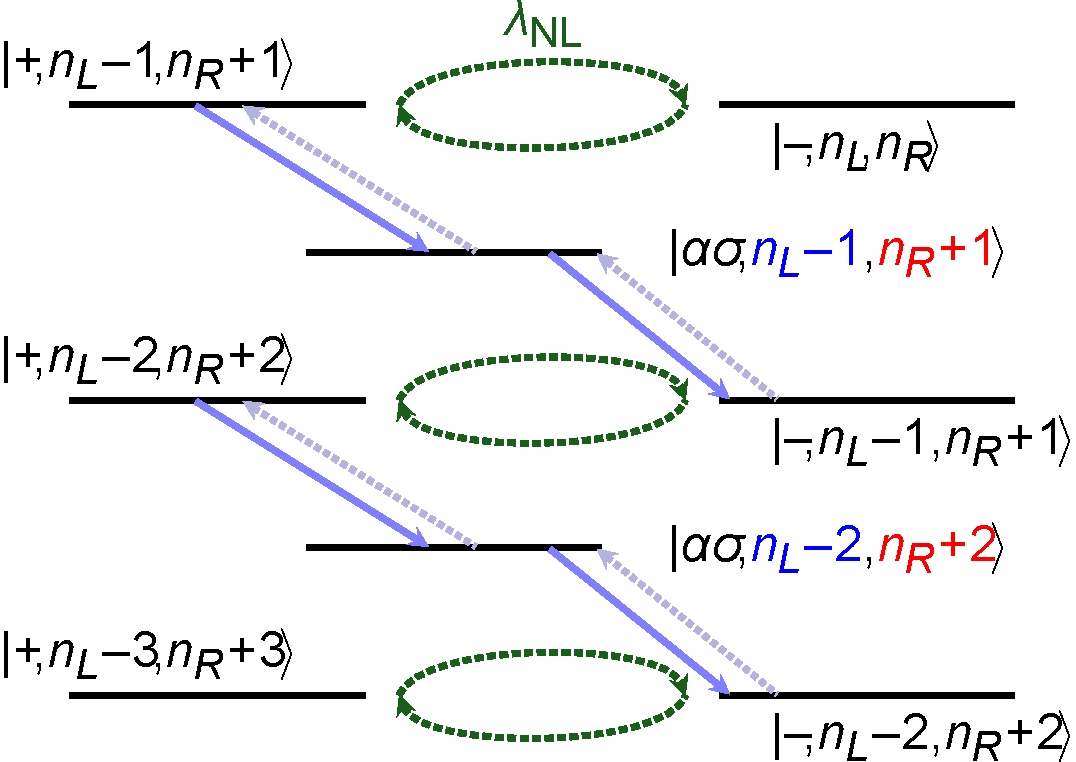
\includegraphics[]{transfer/transfer}
\end{center}
	}
	{\textbf{Electronic current and photon occupation at $\delta \approx 
	\omega_L - 
	\omega_R$:}\\[2ex]
		\begin{center}
			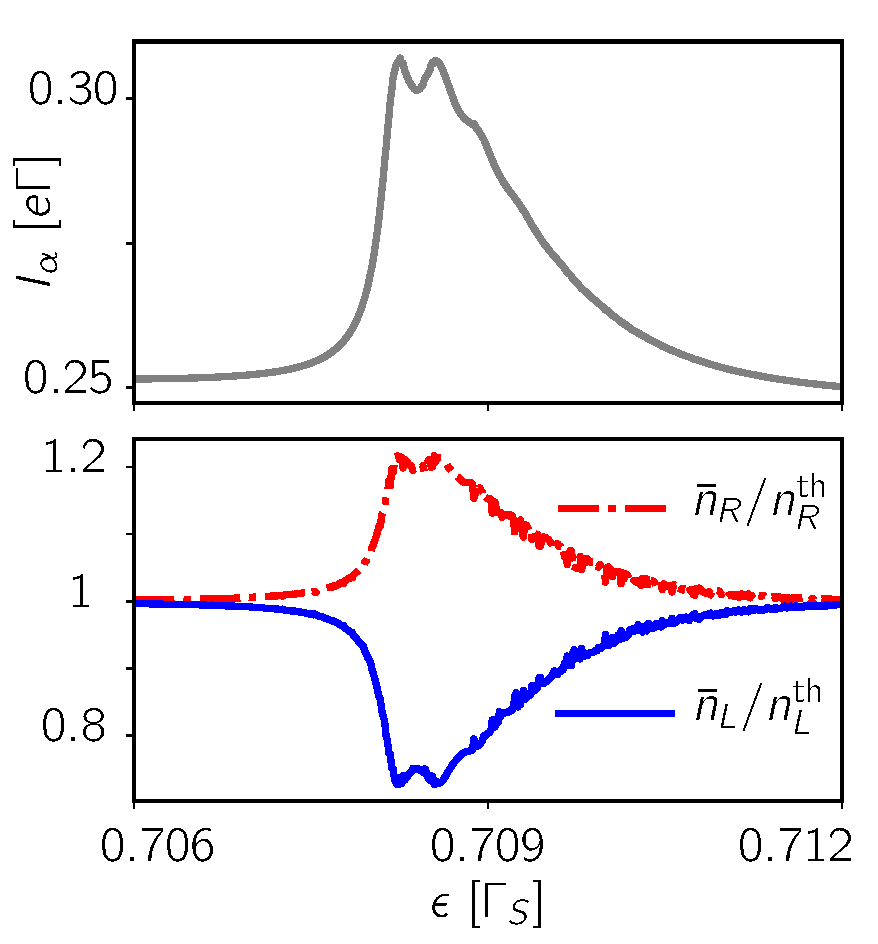
\includegraphics[]{Fig4/Fig4}\\[1ex]
		\end{center}
	\begin{itemize}
		\item The left resonator is \bluebf{cooled down} while the right one 
		is 
		\redbf{heated}
		\item Steady \orangebf{heat flow} between the resonators induced by 
		Cooper-pair splitting
	\end{itemize}
	}
	{\textbf{Heat transfer efficiency (at $\delta \approx \omega_L - 
	\omega_R$):\\[1ex]}
	
	\begin{itemize}
		\item Energy quanta transferred per unit time: $|\dot{E}_L - 
		\dot{E}_R|/(\omega_L - 
		\omega_R)$\\[1ex]
		\item Rate of Cooper-pair injection: $(I_L + I_R)/(2e)$\\[1ex]
		$\Rightarrow$ \greenbf{Efficiency:} $\eta_\mathrm{NL} = \frac{2e 
		|\dot{E}_L - 
			\dot{E}_R|}{(I_L + I_R)(\omega_L - 
			\omega_R)}$\quad(photons transferred per CP)\\[2ex]
	\end{itemize}
	\begin{center}
		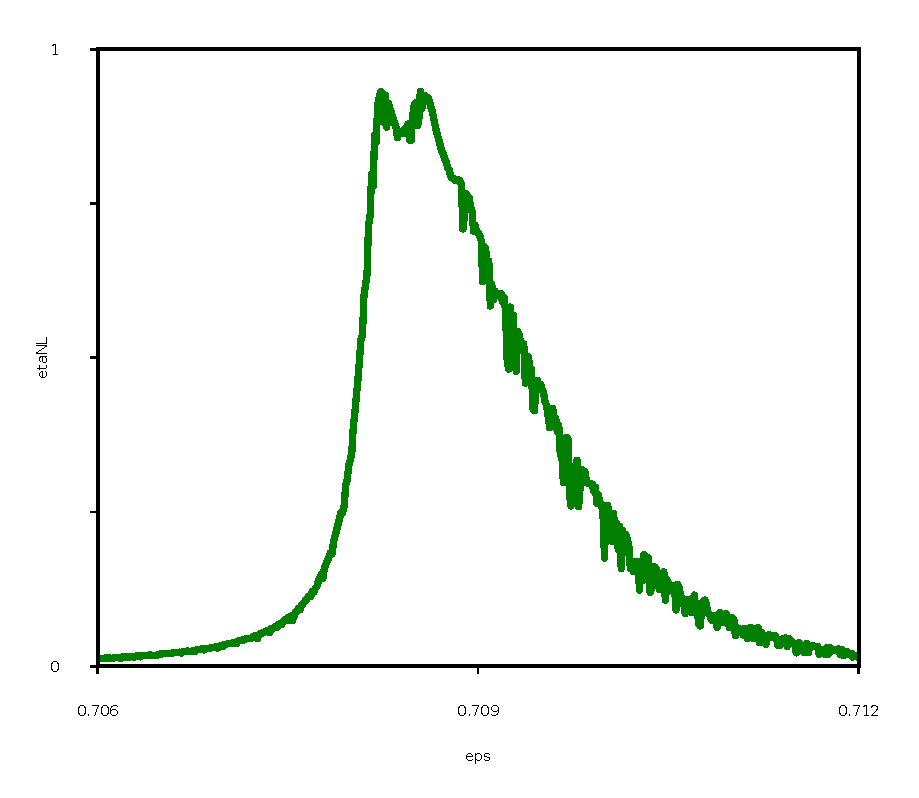
\includegraphics[]{Fig3/Fig3}\\[1ex]
		\greenbf{Near-unity} transfer efficiency!
\end{center}
	}
	{}
	{}
	{}
	{}
	{}
}

%\settoheight{\headerheight}{\phantom{\vbox{\header}}}
\settoheight{\introheight}{\vbox{\introduction}}
\settoheight{\modelheight}{\vbox{\model}}
\settoheight{\coolingheight}{\vbox{\cooling}}
\settoheight{\transferheight}{\vbox{\transfer}}

\begin{textfeld}{\margin}{\margin}
	\header
\end{textfeld}
%\settoheight{\headerheight}{\phantom{\vbox{\header}}}

\begin{textfeld}{\margin}{20.5cm}
	\introduction
\end{textfeld}
%
%\begin{textfeld}{\margin+\blockxsep+29cm}{21.5cm}
%	\model
%\end{textfeld}
%%
\begin{textfeld}{\margin}{21.5cm+\modelheight+\blockysep}
	\cooling
\end{textfeld}
%
\begin{textfeld}{2cm}{21.5cm+\modelheight+\coolingheight+2\blockysep}
	\transfer
\end{textfeld}

%\begin{textfeld}{2cm}{\paperheight - 8 cm}
%	\cdline[thick=12pt]{\paperwidth- 4 cm}
%\end{textfeld}

\vspace*{108cm}
\cdline[thick=12pt]{\paperwidth- 4 cm}
\begin{pframe}[0.5]
	\begin{multicols}{2}
		\printbibliography[heading=none]
	\end{multicols}
\end{pframe}




%\begin{textfeld}{2cm}{\paperheight - 7 cm}%
%%	\begin{fitbox}{0.25\paperwidth}{5cm}
%		\printbibliography[heading=none]
%%		[1] J.J. Viennot, \emph{et al.}, PRB \textbf{89}, 165404 (2014).
%%		
%%		[2] A. Stockklauser, \emph{et al.},
%%		PRX \textbf{7}, 011030 (2017).
%%		
%%		[3] J. Schindele, \emph{et al.}, PRL \textbf{109}, 157002 (2012).
%%		
%%		[4] R. Hussein, \emph{et al.}, PRB \textbf{99}, 075429 (2019).	
%%	\end{fitbox}
%\end{textfeld}%
%
%\begin{textfeld}{2cm+0.25\paperwidth}{\paperheight - 7 cm}%
%	\begin{fitbox}{0.3\paperwidth}{5cm}
%		[5] M. Mantovani, \emph{et al.},
%		arXiv:1907.04308 (2019).
%		
%		[6] A. Rozhkov and D. Arovas, PRB
%		\textbf{62}, 6687 (2000).
%		
%		[7] R. Hussein, \emph{et al.}, PRB \textbf{94}, 235134 (2012).		
%		
%		[8] M. Governale, \emph{et al.}, PRB \textbf{77}, 134513 (2008).
%	\end{fitbox}
%\end{textfeld}%

\begin{textfeld}{0cm}{\paperheight - 7 cm}%

\rightskip8cm \hfill
\begin{fitbox}{30cm}{5cm}
	\begin{flushright}
			
	
\includegraphics[width=26pt]{graphics/website.png}\hskip
	10pt\textcolor{seeblau100}{\textbf{\textit{qt.uni.kn}}}
	

	
\includegraphics[width=26pt]{graphics/twitter_Logo.png}\hskip
	10pt
	\textcolor{seeblau100}{\textbf{\textit{@QtUkon}}}
	

	
\includegraphics[width=26pt]{email.png}\hskip 
	10pt
	\textcolor{seeblau100}{\textbf{\textit{mattia.mantovani@uni-konstanz.de}}}
	% 
	\end{flushright}
\end{fitbox}
\end{textfeld}%

\begin{textfeld}{0cm}{\paperheight - 7 cm}
	\rightskip 2cm
	\hfill
\includegraphics[height=5cm]{qrcps.png}
\end{textfeld}

\end{document}